\documentclass[journal]{IEEEtran}
\usepackage[T1]{fontenc}
\usepackage[utf8]{inputenc}
\usepackage{microtype,cite,listings}
\usepackage{graphicx,booktabs,longtable,tabularx,array,amsmath,xcolor}
\usepackage[hyphens]{url}
\usepackage[colorlinks=true,linkcolor=teal,urlcolor=teal,citecolor=teal]{hyperref}
\hypersetup{pdftitle={BULL II: Binding Authority to Execution},pdfauthor={Luis Minier / Anharmoniclabs},pdfsubject={Revised technical report; validated runtime ab53f56; physical signing blocked}}
\setlength{\parskip}{0pt}
\setlength{\parindent}{1em}
\setlength{\emergencystretch}{3em}
\renewcommand{\arraystretch}{1.18}
\newcolumntype{Y}{>{\raggedright\arraybackslash}X}
\newcommand{\code}[1]{\texttt{#1}}
\newcommand{\repo}[1]{\href{https://github.com/Anharmoniclabs/BULL/blob/ab53f563bcbcaf60820acb318b8212796ce502ff/#1}{\nolinkurl{#1}}}
\newcommand{\ev}[1]{\nolinkurl{#1}}
\title{\textbf{BULL II: Binding Authority to Execution}\\[5pt]\large Implementation, Authenticated Evidence, Controlled Recovery,\\and the Boundary of Physical Approval}
\author{Luis~Minier\thanks{Luis Minier is an independent researcher at Anharmoniclabs, New York, NY, USA. ORCID: 0009-0006-7321-4167. Technical report, September 23, 2026; revision 4. Validated runtime: \texttt{ab53f56}. Prepared in IEEE journal style; not an IEEE publication or peer-reviewed article.}}
\lstset{basicstyle=\ttfamily\scriptsize,breaklines=true,columns=fullflexible,keepspaces=true,showstringspaces=false,frame=single,rulecolor=\color{lightgray},framesep=4pt}
\urlstyle{same}
\interdisplaylinepenalty=2500
\widowpenalty=10000
\clubpenalty=10000
\begin{document}
\raggedbottom
\maketitle
\begin{abstract}
BULL places execution authority outside an AI agent's generated output. Trusted host integration binds a proposed operation to permissions, an exact executable and arguments or broker resource, admitted input bytes, and an active security domain. Mandatory Linux protections and, on the guest route, a fresh QEMU/KVM instance constrain the resulting execution. Authenticated control messages and audit checkpoints distinguish workload output from trusted completion. This report documents the implemented system and the retained local evaluation through clean source \code{ab53f56}: 501 passing tests and 21 passing subtests, all five real-KVM acceptance cases, three bounded formal models, authenticated host and guest receipts, and a source-distribution-to-wheel installation check. A separate historical Qwen run completed 40 fixed read-only actions in 707.4835 seconds with two controlled recoveries and one credential denial; those actions used the host sandbox, not MicroVM execution. Subsequent KB2040 tests witnessed two-click YES and three-click NO diagnostics, and prompted a bounded USB stale-response fix. These events were unsigned. No secure element or production signing key is present, and consequential credential release remains blocked. The paper supplies editable LaTeX, plotted public data, evidence hashes, reproduction commands, and an explicit acceptance matrix. It reports operator-run evidence for identified paths rather than arbitrary-agent security, exactly-once external effects, multi-day reliability, or independent certification.
\end{abstract}
\begin{IEEEkeywords}
AI-agent security, execution governance, capability authorization, information transport, MicroVM isolation, authenticated audit, physical approval, reproducibility.
\end{IEEEkeywords}

\section{Introduction}
An agent's proposal becomes a security decision when an application turns it into a process, network request, or credential retrieval. BULL checks that transition in trusted code. Model output cannot create an installation identity, grant itself permission, mint a production permit, or satisfy a physical approval requirement. The engineering question is whether the operation that actually executes still matches the operation whose authority, input, and protections were checked.

This is a new, source-editable revision of \emph{BULL II: Binding Authority to Execution}. The preceding Zenodo PDF used publication snapshot \code{437de3f} and validation candidate \code{603365e}~\cite{prior}. It reported 489 tests and described the physical gesture attempt as cancelled. That was its recorded scope. This revision incorporates the later software qualification at \code{ab53f56}, successful unsigned gestures at \code{437de3f}, the subsequent USB fix, and session hardening integrated through PR~63. It preserves the source identity of each measurement.

The cutoff is the clean runtime at \code{ab53f56}. New branches or adapters, including the subsequently opened contained-HTTP-honeypot PR~64, are outside this qualification. The documentation commit carrying this paper is not itself the source on which the retained live deployment experiment ran. Future CI results on that documentation commit are separate publication checks.

\begin{table*}[!t]
\centering\small
\begin{tabularx}{\linewidth}{@{}p{0.19\linewidth}p{0.19\linewidth}Y@{}}
\toprule
Evidence unit & Source identity & Scope and result \\
\midrule
September 20 benchmark & \code{cd461ae} & Eleven selected scenarios, three repetitions each; 33 passes. Historical timings only.\\
Historical KVM timing & \code{d218e68} plus recorded patch/tree & One measured allowed run; five separate acceptance cases.\\
Historical Qwen run & \code{974eb17} plus exact dirty-source manifest & 40 host-sandbox actions, two recoveries; 380 tests plus 6 subtests. Commit alone is insufficient.\\
Earlier clean candidate & \code{428db9c} & 437 tests plus 6 subtests; five KVM cases.\\
Integrated candidate & \code{603365e} & 489 tests plus 21 subtests; five KVM cases.\\
Physical diagnostics & \code{437de3f}, BULL-DIAG-3 & Two-click YES and three-click NO observed; manual stale-packet drain before NO. No signatures.\\
Latest qualified software & \code{ab53f56} & 501 tests plus 21 subtests; five KVM cases; hardware signing blocked.\\
\bottomrule
\end{tabularx}
\caption{Distinct evidence units. Counts are neither additive nor a percentage of security coverage. Full hashes and provenance are in the companion.}
\label{tab:identity}
\end{table*}

\section{Security objectives and trust assumptions}
The design follows least privilege and mediation principles described by Saltzer and Schroeder~\cite{E_Saltzer}. Confidentiality, integrity and availability provide the organizing security objectives~\cite{E_FIPS199}; the following maps those objectives to BULL's actual controls.
The untrusted side includes the model's generated text, downloaded content, admitted workload code, and workload output. Trusted components include the administrator, Linux kernel, installed BULL runtime, authority registry, policy/integrity keys, brokers, and deployment configuration. The guest route additionally trusts QEMU/KVM, firmware, the guest kernel, and the trusted guest supervisor. External checkpoint authentication depends on collector operation and key custody. A compromised host administrator with access to those keys remains inside the current trust boundary~\cite{claims}.

Confidentiality depends on scoped reads, admitted read-only inputs, restricted network visibility, and controlled secret/egress brokers. Integrity depends on binding a request to the exact effect, preserving the admitted bytes, authenticating control traffic, consuming approval once, and maintaining checkable audit history. Availability depends on finite budgets, deadlines, cancellation, descendant cleanup, and explicit recovery rules. An allowed action can still be harmful within its granted authority; broad read and send grants can authorize disclosure.

For an execution request $r$, the intended contract is
\[
\begin{aligned}
\operatorname{Execute}(r)\Rightarrow{}&\operatorname{Allowed}(r)\land\operatorname{Bound}(r)\\
&{}\land\operatorname{Admitted}(r)\land\operatorname{Protected}(r).
\end{aligned}
\]
For a consequential broker effect, current approval and required audit delivery are additional conditions. This notation states the contract exercised by the implementation and selected tests; it is not a proof about every possible Python integration or hostile kernel.

Domains carry host-owned identities and bounded capabilities. A child's capabilities and egress hosts are subsets of its parent's. Siblings remain distinct while contributing to shared root-domain behavioral history. A freeze must remain effective after an approval request is created. Provenance describes origin; it does not confer authority. Advisory monotonicity and development orchestration are separate from the production enforcement described below.

\section{Execution architecture}
\subsection{From proposal to admitted bytes}
\code{ProductionDispatcher} combines an untrusted proposal with a trusted context. Resource canonicalization, capability checks, domain state, and history determine whether an exact operation is allowed. Process launch needs \code{process.exec}; permission to read a file does not authorize shell execution. A permitted executable does not authorize a modified argument vector. The runtime accepts a dispatcher-minted permit bound to the operation it will perform~\cite{runtime}.

File admission securely traverses the selected project, copies eligible inputs to private snapshot storage, verifies the copy, scans it with ClamAV, and rehashes the admitted content. Unsupported file objects and changes that invalidate identity are refused. The workload sees the admitted snapshot, not a mutable source project. Directory storage-size normalization permits content comparison across filesystems while preserving file hashes, sizes, and source race checks. Trusted runtime code is kept separate from admitted workspace data.

\begin{figure*}[!t]
\centering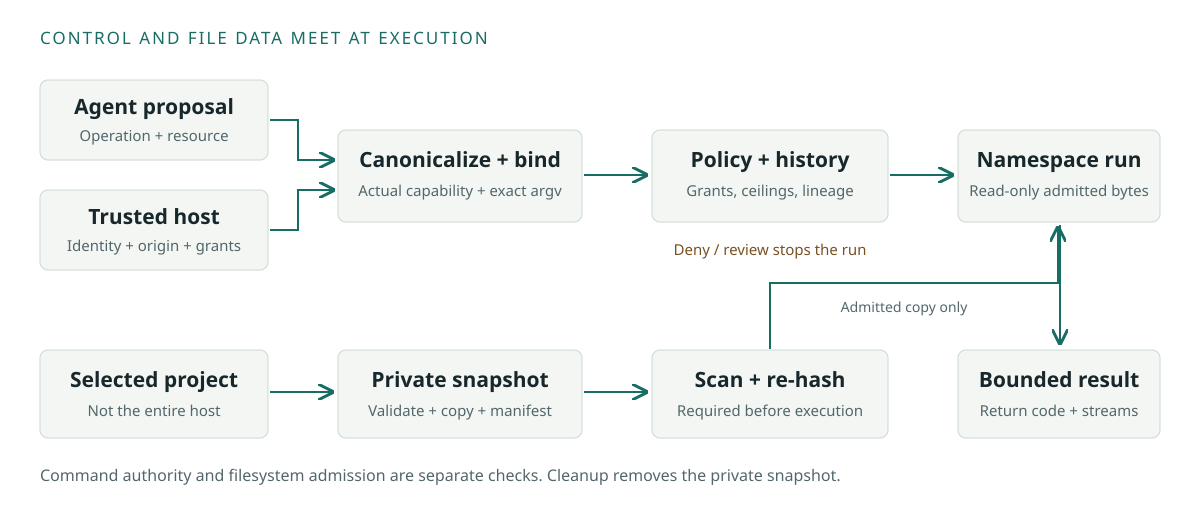
\includegraphics[width=\linewidth]{figures/data-flow.pdf}
\caption{Repository control and file-data paths. The companion preserves the original SVG and its source hash. Authority and admitted input converge before execution; this is an architecture diagram, not measurement evidence.}
\end{figure*}

\subsection{Linux protection before workload release}
The namespace route combines user, mount, PID, network, and IPC namespaces; read-only mounts; \code{no\_new\_privs}; strict seccomp; Landlock; and cgroup v2 budgets. The parent does not release the workload solely because the launcher started. Trusted bootstrap code installs protections and sends nonce-bound evidence through a private pipe. The parent checks the expected privilege state, seccomp profile, PID namespace, Landlock, and network conditions, then acknowledges the pre-exec gate. The workload does not inherit the evidence descriptor. This is a checked software bootstrap, not hardware attestation~\cite{linux,runtime}.

Qualification observes enforcement rather than only configuration. The memory probe touches pages under a 64 MiB limit and requires OOM evidence. The process probe attempts bounded forks under a four-process cgroup ceiling. The CPU probe performs one second of work under a 25\% quota. Timeout and cancellation checks require cleanup of owned descendants. These are acceptance-probe settings; production workload limits are separately configured. Security-critical assertions that optimized Python could remove were replaced with explicit exceptions. Eight invalid cases and one valid control across four Python modes produced 36 software cases in the recorded corrective work.


\begin{figure*}[!t]
\centering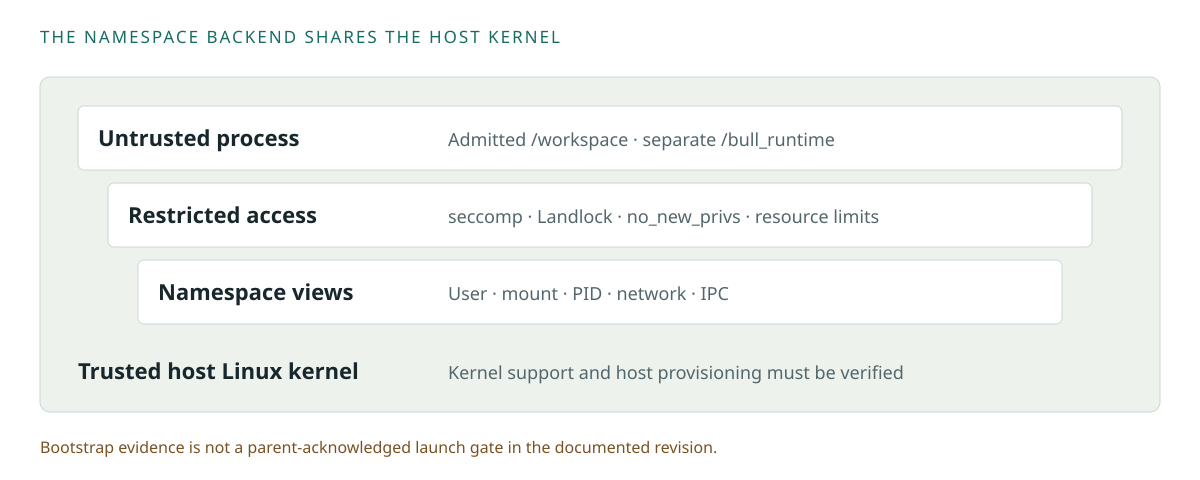
\includegraphics[width=0.92\textwidth]{figures/kernel-layers.pdf}
\caption{Original repository drawing of the nested enforcement layers. Its bootstrap footnote records an earlier design state; the qualified runtime now uses parent validation before release, as described in Section III-B.}
\end{figure*}
\subsection{Fresh one-shot guests}
The QEMU \code{microvm} route adds a separate kernel and hypervisor boundary~\cite{qemu}. The supported guest uses three read-only ext4 inputs: root, admitted workspace, and trusted runtime. It has no guest NIC and no QEMU monitor. Development 9P sharing is an explicit separate option. The launcher validates pinned assets and private session channels; the guest supervisor validates trusted runtime and deployment authority before dispatch. Completion requires authenticated result and audit evidence. The host tracks and reaps its exact QEMU child.

Every qualified guest request starts a fresh VM. A successful fresh guest after a cancelled guest demonstrates a new one-shot session. It does not recover guest RAM, preserve a running process, or retry an uncertain consequential effect. The five KVM outcomes remain distinct from host-only protocol regressions.

\begin{figure*}[!t]
\centering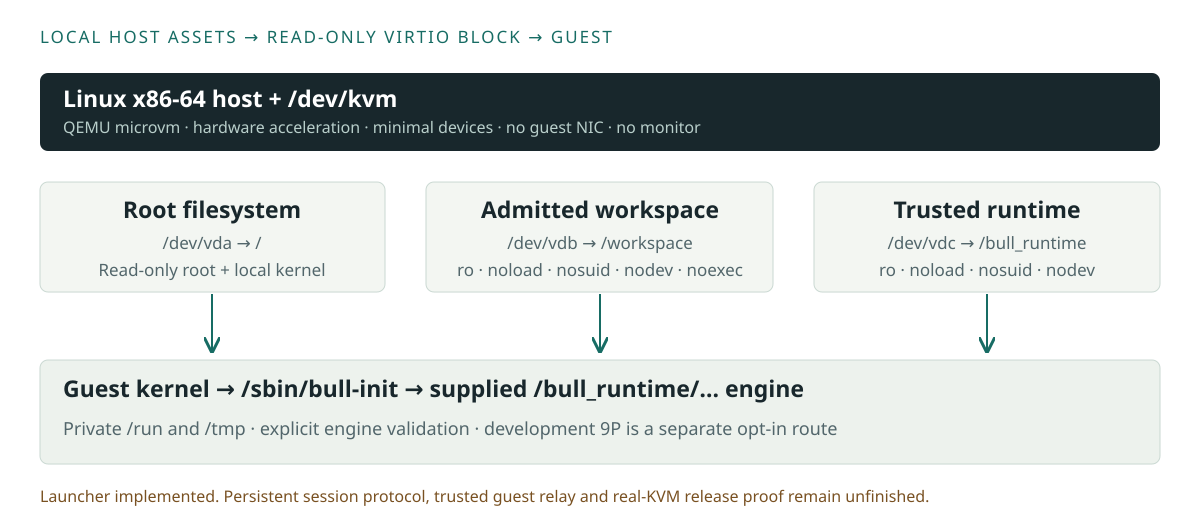
\includegraphics[width=\linewidth]{figures/microvm-io.pdf}
\caption{Original repository drawing of read-only guest inputs and separate control/audit routes. The footer records an earlier state: authenticated one-shot transport and five real-KVM cases are now demonstrated; persistent sessions remain unfinished.}
\end{figure*}

\subsection{Implemented integration inventory}
The implementation exposes several entry paths. Table~\ref{tab:entrypoints} distinguishes production-mediated paths from development orchestration and evaluation interfaces.

\begin{table*}[!t]
\small\begin{tabularx}{\linewidth}{@{}p{0.28\linewidth}YY@{}}
\toprule Entry point & Enforcement & Qualified scope \\
\midrule
Governed local-model adapter & Dispatcher/runtime in host namespace sandbox & Fixed \code{inspect} and \code{checksum}; trusted supervisor and Ollama.\\
Guest engine & Dispatcher/runtime in fresh KVM guest & Host-authorized exact command and one session; five real cases.\\
Dispatcher API & Host-owned exact authority and command & Integrating applications must mediate their actual effects.\\
\code{MultiAgentSystem} & Development callables run in host Python & Bus/policy/canary tests; not automatically a production adapter.\\
CLI/sentinel & Evaluation and advisory interfaces & No independent production-containment claim.\\
External frameworks & Adapter-specific work required & No blanket arbitrary-agent support.\\
\bottomrule
\end{tabularx}\caption{\label{tab:entrypoints}An orchestration test is not evidence that an external adapter's effects use production enforcement.}
\end{table*}

\section{Authenticated transport and evidence}
\subsection{Bounded control frames and session failure}
Control traffic uses a four-byte big-endian length followed by canonical JSON. Fields bind protocol version, session, sequence, kind, payload, and MAC. Supported kinds are \code{ready}, \code{execute}, \code{result}, and \code{error}. Length must be between 1 and 65,536 bytes. Authentication is direction-separated; sequence and session are checked before accepting the payload. A workload's printed status remains data~\cite{transport}.

The later session hardening is included in \code{ab53f56}. A channel records whether execution authority has been used and whether a send or receive operation failed. An exception makes that channel unusable. The host may send one execute request; the guest may receive one. A second execute with a fresh sequence is still refused. A timeout followed by a late result cannot restore the failed channel. An invalid message followed by a valid one cannot restore it either. Fresh-channel zero-length and oversized-frame tests preserve actual framing coverage rather than accidentally hitting only the failed-channel guard.

These checks do not introduce persistent sessions. Requirements for reuse, writable exports, and hostile-host confidential computing are documented separately. Persistent operation would need per-action fresh authority, serialized dispatch, generation binding, cleanup evidence, and reconciliation. Writable publication would need bounded quarantine, safe file types/paths, immutable approved manifests, and crash-safe publication. None of those future interfaces is qualified by the one-shot session tests.

\subsection{Audit checkpoint ordering}
HMAC supplies keyed message authentication~\cite{E_HMAC}. In BULL, its role is to authenticate checkpoint and acknowledgment fields within the deployed trust arrangement; it does not make a compromised producer trustworthy.
The local audit ledger is hash-linked. Authenticated external checkpoints bind an installation/session, record count, and head hash; the client verifies the acknowledgement. Guest audit traffic uses a dedicated trusted relay, separate from workload output and control. An authenticated result alone does not substitute for the required completion evidence. Figure~\ref{fig:audit} shows the repository's evidence route.

\begin{figure*}[!t]
\centering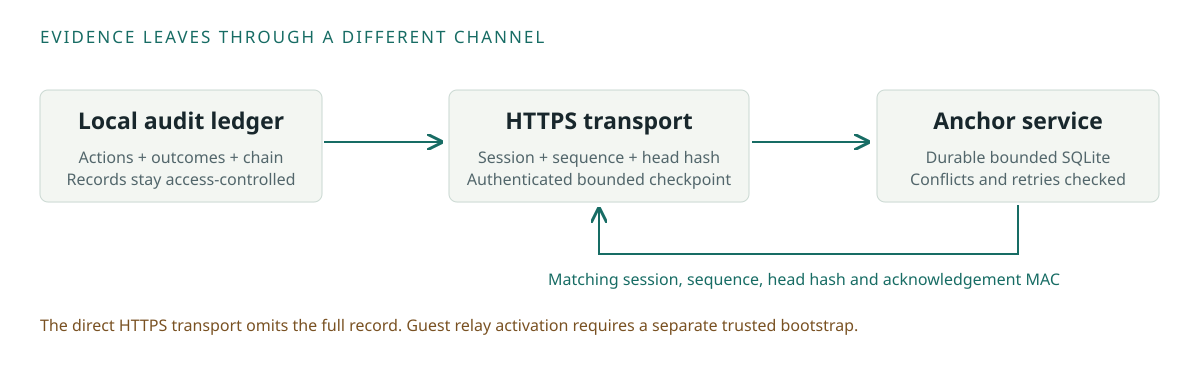
\includegraphics[width=\linewidth]{figures/audit-flow.pdf}
\caption{Local history, guest relay, and external checkpoint flow. Authentication establishes acceptance by the configured authority; it does not independently prove collector retention or a trustworthy compromised host.}
\label{fig:audit}
\end{figure*}

If a local append succeeds but checkpoint delivery fails, subsequent appends stop. Explicit reconciliation retries delivery of the already produced evidence. It does not repeat workload execution. The September 20 external test retained one interrupted record, reconciled it, accepted another authenticated checkpoint, and verified the final two-record ledger. Cloudflare initially rejected Python urllib's default client signature; the documented client user agent reached the Worker. The correction preserved authentication checks.

The existing live collector and the failed preview are different deployment outcomes. The existing collector passed host and guest receipt checks at \code{ab53f56}. The preview identified in the historical Qwen summary returned HTTP 409 at its first authenticated checkpoint and was not promoted. The site deploys from \code{main}; the audit worker retains its separate operator-selected branch. The main-attached \code{bull-audit} build check still reported failure; saved local credentials could not retrieve detailed logs. That failure is retained, not folded into the six successful GitHub validation workflows.

\section{Approval bound to one exact effect}
\subsection{Gate ordering and at-most-once consumption}
Human approval supplements an already permitted consequential action. Implemented protected broker paths include scoped network requests and credential retrieval. The request binds the session, action, resource, parameters, policy, nonce, and expiry. The final gate verifies an enabled enrolled credential and exact binding, consumes the request, advances the custom provider's per-key counter atomically in SQLite, delivers the required approval audit event, rechecks current policy/domain authority, and attempts the broker effect~\cite{approval}.

SQLite provides a local transaction boundary under its storage assumptions~\cite{sqlite}. It does not atomically commit a remote service's side effect. If audit delivery fails after consumption, the approval remains spent. A broker failure after a possible effect is recorded as uncertain; the signature cannot be reused to retry. This establishes at-most-once authorization consumption, not exactly-once remote delivery.

The existing OpenSSH security-key path retains its application and signed user-presence/user-verification requirements. The custom P-256 provider is integrated into the same \code{ApprovalGate}. Enrollment aliases do not reset replay state because counters follow the public-key fingerprint. Skipped counters are accepted; a lost delivery may already have consumed a device counter. Equal or older counters are rejected. Signed denial is terminal and audited. Synthetic keys exercise these software paths; they are not production device credentials.

\subsection{BULL-AUTH-1 encoding and verification}
The implemented codec uses fixed-width big-endian fields, rather than arbitrary JSON formatting. A request is 284 bytes: protocol prefix/type, eight 32-byte fields, and creation/expiry timestamps. The fields bind request ID, session, full action, operation, resource, parameters, policy, and fresh nonce. The maximum lifetime is 30 seconds. SHA-256 of the canonical request identifies the approved request.

The assertion is 240 bytes: protocol prefix and decision, five 32-byte fields, a 32-bit counter, and a fixed 64-byte P-256 signature in $r\Vert s$ form. The fields bind enrolled device identity, request ID, request digest, session, and nonce. ECDSA-SHA256 covers the canonical assertion bytes before the signature. Both structures fit the 512-byte ceiling. Disabled or unknown enrollment, malformed data, wrong binding, expiry, invalid signature, replay, stale counter, changed policy/action/domain, and unavailable required audit must refuse the effect.

There are 24 stateless verifier cases and 23 durable-gate cases in the qualified software suite. They cover synthetic valid approval/denial, invalid and mismatched assertions, persistence, counter aliases, concurrent consumption, and audit-failure behavior. These counts are subsets of the 501 tests, not extra tests to add to that total. The full physical acceptance matrix remains separate.

\section{BULL Hardware Authority: witnessed diagnostics and unfinished signing}
\subsection{What was connected and observed}
Only an Adafruit KB2040/RP2040 was connected. It reported BULL-DIAG-3, \code{approval\_available=false}, no valid ATECC wake response, and no pending request at final inspection. The operator confirmed that no secure-element breakout was present. No production private key was generated, exported, provisioned, or enrolled.

The diagnostic firmware exposes vendor-defined USB HID status and physical input, with no keyboard emulation, mass storage, shell, CDC console, or REPL. It contains no production signing key. Its responses cannot satisfy the approval verifier. The diagnostic firmware built with Pico SDK 2.2.0; the retained successful build source is \code{603365e}, whose firmware tree is identical to that in \code{ab53f56}. C state-machine simulations passed. These are build and simulation results, not signed physical acceptance.

\subsection{Physical sequence and the USB correction}
The initial gesture attempt returned CANCELLED. A retry found the exact USB board in RP2 Boot mode; it was restarted into its installed application without flashing. With the unmodified host CLI at \code{437de3f}, two BOOT clicks returned YES. The first NO attempt rejected a mismatched challenge. A one-off read-only helper drained one queued status reply; then three BOOT clicks returned NO. The successful tests used distinct challenges and ended with no pending request.

The original CLI sent CANCEL during cleanup without consuming its status response. That queued reply could be read by the next invocation. The manual helper used before NO is preserved with its hash in the companion. The subsequent automatic fix drains at most eight validated diagnostic packets, with a 100 ms timeout per receive, before issuing a new command. It rejects malformed, oversized, unexpected-authority, and nonsettling queues, and preserves strict matching to the newly armed challenge. Eight simulated transport tests and two live read-only status queries validated the later fix. The successful physical gestures are attributed to the original CLI plus manual preparation, not retroactively to the automatic fix.

The BOOT prototype maps two clicks to YES and three to NO, with 30 ms debounce and a 600 ms quiet window after the second release. Abandoned or expired requests cancel. Idle clicks confer no future approval. These are unsigned observations of physical input. No cryptographic assertion or protected broker effect was produced.

\subsection{Required production token and trust boundary}
The planned token pairs the KB2040 with a supported secure element and distinct normally-open YES/NO buttons. The intended wiring is 3.3 V/common ground, SDA/D12 and SCL/D13 for I2C, D4 for YES, and D5 for NO. Exact part voltage and configuration must be checked before power or irreversible provisioning. The private P-256 key must be generated inside the secure element and remain non-exportable. The secure-element driver, configuration self-test, signing firmware, authenticated request transport, and witnessed enrollment are unfinished~\cite{hardware}.

Production YES requires a fresh deliberate hold of at least 750 ms after release/debounce; a stable NO denies. Simultaneous buttons, missing protection, secure-element failure, expiry, disconnect, or reset must not authorize. Host cancellation may cancel only. There must be no host YES button, keyboard approval shortcut, software-key fallback, preapproval state, or approval cached for later actions. Signed APPROVE, signed DENY, and replay rejection must all be demonstrated through the existing production gate before acceptance.

The RP2040 lacks the hardened authenticated firmware trust assumed of a commercial authenticator. A secure element protects key extraction but cannot by itself prove that compromised controller firmware required a human. The no-screen prototype trusts the host's presentation of the requested action. Request binding does not establish that the human saw trustworthy action text. The prototype is not FIDO2-certified, tamper-proof, equivalent to a commercial security key, or qualified against invasive physical attacks. A future controller with verified boot and a trusted display could address parts of this boundary; it is not implemented here.

\begin{table*}[!t]
\small\begin{tabularx}{\linewidth}{@{}p{0.46\linewidth}Y@{}}
\toprule Acceptance group & Recorded state \\
\midrule
Boot, diagnostic HID, no approval key/fallback & Observed diagnostic status; no authority available.\\
Physical BOOT YES/NO & Witnessed unsigned two-/three-click results at \code{437de3f}; retained failed attempts.\\
Separate YES hold / NO / simultaneous inputs & C simulations; physical wiring and ceremony pending.\\
Host digest, nonce, session, identity, expiry and signature binding & Software verifier/gate tests pass using synthetic signatures.\\
Atomic request/counter consumption; signed denial audit & Implemented and software-tested; physical signing pending.\\
Secure element, internal key generation, non-exportability & Blocked: no secure element installed.\\
Public-key enrollment into trusted production policy & No production token enrolled; disabled public records grant no authority.\\
Authenticated signing HID, counter/sign-failure handling & Production firmware and device acceptance unfinished.\\
Physical signed approval, denial, replay, drift, expiry & Not demonstrated.\\
Physical disconnect/reset/timeout/fault matrix & Simulations/host checks only; full device acceptance pending.\\
Protected credential release & Blocked.\\
\bottomrule
\end{tabularx}\caption{Grouped hardware acceptance requirements. Passing diagnostics does not close the secure-signing gate. Detailed requirements remain in the archived hardware design.}
\end{table*}

\section{Evaluation method and results}
\subsection{Latest clean-source qualification}
The retained release record identifies clean \nolinkurl{ab53f563bcbcaf60820acb318b8212796ce502ff}~\cite{evidence}. It records 501 passing tests and 21 passing subtests, no failures and no skips. Compilation, diff validation, three TLA+ parse/model gates, wheel/distribution checks, site build, and unchanged-clean-source checks passed. The local full pytest invocation took 13.089 seconds; this is suite duration, not per-action latency. GitHub's publication run reported its own 18.59-second suite duration, not an additional experiment to average with the local run.

All six recorded GitHub workflows succeeded on this source: security regression, MicroVM host regression, formal invariants, public guest recipe configuration, Pages publication, and FreshClam guest database integration. Python 3.11/3.13 CI supplements the local Python 3.14.7 environment. Source, strict-host, cgroup delegation/enforcement, signed production/deployment configuration, local TLS, external host/guest receipts, pinned guest assets, KVM readiness/current cases, and unchanged-source gates passed. The hardware approval gate remained BLOCKED; the deployment checker therefore did not report an all-gates release success.

\begin{figure*}[!t]
\centering\includegraphics[width=0.85\textwidth]{figures/regression-milestones.pdf}
\caption{Counts from retained machine-readable records. Bar lengths show tests; labels list subtests separately. Increasing counts do not measure attack-space coverage.}
\end{figure*}

\begin{table}[ht]
\small\begin{tabularx}{\linewidth}{@{}p{0.25\linewidth}Y@{}}
\toprule Real-KVM case at \code{ab53f56} & Required observed outcome \\
\midrule
Allowed & Authorized workload executed and trusted completion was accepted.\\
Denied & Refusal before workload execution.\\
Timeout & No successful completion accepted; owned work cleaned up.\\
Cancellation & Exact guest child reaped; interrupted work not relabeled complete.\\
Missing protection & Required protection failure stopped admission.\\
\bottomrule
\end{tabularx}\caption{All five passed with the pinned guest assets. A subsequent fresh allowed guest also passed as a distinct session.}
\end{table}

The fixed-tool deployment check executed both inspect and checksum through production dispatch and denied an empty-grant request without execution. A fresh guest after cancellation passed. Packaging built a wheel from the source distribution, installed it in a fresh environment outside the checkout, and recorded artifact digests. No new forty-action model run was performed at \code{ab53f56}.

\subsection{Historical selected defensive corpus}
At \code{cd461ae}, eleven selected defensive scenarios ran three times each: 33 passes and zero failures. The recorded host was Linux 7.2.6-1-cachyos x86\_64, Python 3.14.7, AMD Ryzen 5 7430U with 12 logical CPUs, and 11 GiB memory. End-to-end pytest means range from 292.603 to 376.640 ms and include interpreter, fixture, and process startup. Peak RSS ranges from 44.668 to 46.086 MiB. The corpus is deliberately selected; its 100\% result is not a broad malicious-effect probability or false-denial estimate.

\input{benchmark-table.tex}
\begin{figure*}[!t]
\centering\includegraphics[width=\textwidth]{figures/defensive-corpus.pdf}
\caption{Selected defensive corpus at cd461ae: mean pytest duration and recorded minimum--maximum across three runs per scenario. All 33 selected runs passed. These intervals include test-harness overhead; they are not confidence intervals.}
\end{figure*}


The separate 500-iteration in-process loops recorded 4.897 microseconds per traversal rejection, 66,559.856 microseconds per prompt-injection denial, and 438,559.052 microseconds per benign multi-agent allow. The last two reused one \code{MultiAgentSystem}, accumulating trace/honeytoken state. They describe that construction, not a fresh-state policy latency comparison, an isolated component cost, or a production-adapter throughput claim.


\begin{figure*}[!t]
\centering\includegraphics[width=\textwidth]{figures/hotpath-results.pdf}
\caption{Recorded 500-iteration loops at cd461ae. The logarithmic axis preserves the measured scale. Prompt-injection and benign multi-agent loops reused state; they are not comparable fresh-instance policy microbenchmarks.}
\end{figure*}
\subsection{Historical MicroVM timing}
The retained September 20 guest measurement used \code{d218e68} plus its recorded local patch and source-tree hash. QEMU process start to dispatcher-ready was 12,157.320 ms; launcher invocation to readiness was 12,282.303 ms. Guest runtime/dispatcher initialization was 597.739 ms; dispatch including admission/scanning was 9,165.705 ms; sandbox setup to trusted pre-exec was 308.901 ms; pre-exec to reap was 99.492 ms. The fixture body reported 0.476 ms, completion audit acknowledgement 33.714 ms, and result/audit overhead outside dispatch 34.355 ms. These intervals overlap and must not be summed. There is one observation, no percentile estimate, and no new timing claim for \code{ab53f56}.


\begin{figure*}[!t]
\centering\includegraphics[width=\textwidth]{figures/kvm-results.pdf}
\caption{Historical single-run QEMU/KVM intervals from the retained September 20 report. Intervals overlap and must not be summed. Logarithmic scale; no inferred percentiles or repeated-run distribution.}
\end{figure*}
\subsection{Historical local-model run}
The model was \code{qwen2.5:1.5b-instruct}, identified by its full digest in the companion. Trusted code provided the fixed tools, resource paths, arguments, grants, and identity. The model returned untrusted JSON selecting inspect/checksum. The recorded prompt explicitly exercised both tools after an earlier prompt repeatedly selected one.

The run completed 40 actions in 707.483500783 seconds, with two recovery events, one credential denial, 130 ledger records, a locally verified authenticated receipt, and no pending plan. The backend was host \code{NamespaceSandbox} via \code{ProductionDispatcher} and \code{ProductionRuntime}. Ollama and the supervisor were trusted host processes. None of the forty actions ran inside a MicroVM. Five KVM cases in that historical bundle were separate tests against a disposable local TLS collector; the agent run used the existing live collector.

The first dedicated worker persisted a plan and exited with code 75 before dispatch. The next recovered the plan, executed the read-only action, and exited with code 76 before recording completion. A third invocation recovered and finished. Completed steps were preserved; incomplete read-only work could run again. A fresh reconstructed deployment separately completed two actions with two recoveries and one credential denial in 36.60895827 seconds. The historical regression was 380 tests plus six subtests. Its source was a dirty worktree at base \code{974eb17}; the included file-hash manifest is required to identify it. Offline reconstruction is not a claim that the base commit alone reproduces the run.

\subsection{Controlled failures and recovery}
Seven controlled cases exercise four combinations of injected ENOSPC/EIO at append/head-write boundaries, a ledger storage budget, worker exit with a pending plan, and disposable TLS collector outage/restart with retained SQLite state. An append failure before writing preserves a valid history. A record written before its trusted head can advance leaves inconsistent evidence and blocks further appends. The storage-budget test refuses an additional record without a partial append. The worker releases its lock on exit while preserving the pending plan.

The collector test stops only its own loopback server, observes delivery failure and blocked advancement, restarts against retained state, explicitly reconciles, verifies idempotent checkpoint retry, and continues to three accepted records. Storage errors are injected; no physical disk controller failure or host power loss is reproduced. The production collector was not subjected to a disaster-recovery exercise. No host reboot or multi-day run is claimed.

\subsection{Formal models and supplemental review}
TLA+ specifies state transitions and invariants~\cite{E_Lamport}. The finite BULL models cover runtime, session/audit, and approval transitions. The recorded model sizes are 405, 57, and 112 distinct states respectively. All parse/model gates passed. They check the configured finite specifications, not an automatically established refinement from all Python code or every environment to the model.

The standalone adversarial harness recorded 49 source/API probes. Corrections made it recognize a normal \code{executed=false} denial, use legitimate full argument vectors for positive controls, and preserve forwarded hop history. It does not replace live kernel/guest acceptance. A downloaded GLM/Perplexity pentest script was inspected before its read-only static, hygiene, and invariant suites were invoked. Its main routine incorrectly constructed suite objects. Reported example-environment values were public placeholders, and its legacy branch-protection lookup missed active rulesets. Neither observation was relabeled a secret leak or missing repository protection. This was a supplemental script review, not an independent live penetration test.

\section{Corrective work and retained failures}
The implementation record includes failures because they explain what the passing cases actually tested. Guest bring-up corrected literal parsing of digit-bearing configuration keys, qboot/non-ACPI setup, and AMD SSBD feature dependencies without suppressing enforcement. The guest gained required Bash, ClamAV, Python modules, utilities, and verified databases. A database-path mismatch received an immutable alias. Actual library loading replaced an unreliable \code{find\_library}-only test. Scanner loading needed a 1536 MiB ceiling in the historical run, separate from its 512 MiB workload limit.

Snapshot identity was corrected for filesystem-dependent directory sizes, and isolated snapshot-worker imports were anchored to the trusted runtime. Private-file fixtures were given explicit owner-only modes instead of weakening runtime permission checks. Resource probes were corrected to charge memory and test forks inside a dedicated cgroup rather than measuring unrelated UID-wide desktop pressure. Optimized-Python assertions became explicit errors. Hardware linking added the required \code{pico\_unique\_id} dependency. USB stale-response handling and one-shot channel failure semantics were corrected as described above.

Earlier validation attempts lacked build/scanner prerequisites, timed out a guest scanner, lost an audit relay, or exceeded Linux's Unix-socket path limit. The final unchanged-candidate checks used verified prerequisites and a shorter private output path. PR~61's restricted environment recorded 488 passes plus 21 subtests and four failures; the same four reproduced on its untouched baseline, and that environment had no KVM. Those historical failures remain in its archived report. The later \code{ab53f56} full-host qualification passed; it does not rewrite the earlier environment's outcome.

\section{Reproduction, distribution, and publication}
\subsection{Software and deployment reproduction}
Use a supported Linux host and keep evidence directories outside the checkout. The following pins the runtime that produced the latest retained live results:
\begin{lstlisting}
git clone https://github.com/Anharmoniclabs/BULL.git BULL-runtime
cd BULL-runtime
git checkout --detach ab53f563bcbcaf60820acb318b8212796ce502ff
python3 -m venv .venv
.venv/bin/python -m pip install -e '.[test,hardware]' 'setuptools>=77' wheel
.venv/bin/python tools/release_check.py \
  --tla-jar /ABS/PATH/tla2tools-1.7.4.jar --output /tmp/bull-src-01
\end{lstlisting}
Java and the repository-pinned TLA+ 1.7.4 jar are required. Preserve dependency resolution and the host environment with the report. Source tests do not substitute for namespace, Landlock, seccomp, scanner, delegated cgroup, KVM, and real collector prerequisites. The core Python package has no mandatory third-party Python runtime dependencies; test/hardware extras include cryptography. The qualified custom-provider dependency range is \code{cryptography>=43,<51}.

Follow \repo{docs/REPRODUCIBLE_DEPLOYMENT.md} for host setup and a new installation. The initializer creates private state outside Git, independent policy/integrity/collector keys, and installation/session identities; it refuses an existing state directory. Directories are owner-only and private files use mode 0600. Do not copy another operator's private deployment keys to reproduce the paper. Supply the new installation's collector endpoint and checked guest assets, then run:
\begin{lstlisting}
.venv/bin/python tools/deployment_check.py \
  --deployment /ABS/PRIVATE/deployment \
  --tla-jar /ABS/PATH/tla2tools-1.7.4.jar --output /tmp/bull-dep-01
PYTHONPATH=src .venv/bin/python microvm/integration.py \
  --kernel /ABS/PRIVATE/bzImage --rootfs /ABS/PRIVATE/rootfs.ext4 \
  --firmware /ABS/PRIVATE/qboot.rom \
  --output /tmp/bull-kvm-01 --case all --cpu-profile host
\end{lstlisting}
The standalone guest runner uses a disposable TLS collector by default. Its external collector options select a separate installation-owned destination. Keep output paths short because the runner creates Unix sockets. Record source cleanliness, guest/runtime hashes, sessions, environment, gates, and retained failures. Missing hardware should remain BLOCKED.

For a new model run, initialize a separate deployment admitting \code{examples/governed-agent}, with the documented read/process ceiling, delegation, scanner, and collector. Install the selected Ollama model and preserve its digest. Run:
\begin{lstlisting}
.venv/bin/python tools/check_governed_agent.py \
  --deployment /ABS/PRIVATE/agent-deployment --output /tmp/bull-agent-01 \
  --model qwen2.5:1.5b-instruct --steps 40 --interval 5 \
  --max-seconds 7200 --enter-coordinator
\end{lstlisting}
Verify expected outputs, both tools, sandbox evidence, worker exit phases, credential denial, authenticated receipt, and an empty pending-plan state. \code{tools/audit\_governed\_agent.py} checks the retained ledger; an independently held expected head strengthens comparison. A new run is new evidence, not a reproduction of old random/session identifiers.

\subsection{Exact guest and package identities}
The qualified guest assets are those in Table~\ref{tab:hashes}. The public \code{guest-2026-09-22} release supplies source/license materials alongside unchanged image assets~\cite{distribution}. Reconstruction matched recorded inputs and resolved configurations, including all 67 package/version entries in the original build log. Offline preparation and verification of 57 source archives passed with external networking unavailable. A full offline recompilation and two independent byte-identical guest builds have not been demonstrated.

\input{hashes-table.tex}

The release candidate supplies a full Git source archive, Python source distribution, wheel built from that distribution, release notes, hardware acceptance status, validation JSON, and checksums. All seven uploaded draft assets were verified against local hashes. It remains a draft prerelease: software qualification is not a stable-release or physical-approval certification. Original source retains GPL-2.0-or-later; upstream dependencies and supplied guest materials retain their notices. The process is an engineering distribution check, not independent legal certification.

\subsection{Paper companion and publication state}
This revision includes native \code{paper.tex}, a reproducible build script, exact Python build dependencies, original repository SVGs, generated figure inputs, a source/evidence manifest, a requirement-to-evidence map, and sanitized records. The build verifies every archived input hash before producing the PDF and companion ZIP. It generates tables, regression milestones, defensive-test intervals and hot-path plots from retained JSON/CSV; the KVM plot is extracted from the archived measurement table. No synthetic observations are added. The companion includes its own checksum manifest. Rebuilding the paper requires the documentation revision containing these files, whereas rerunning the qualified runtime uses the pinned revision above.

The evidence archive contains aggregate public records, not private collector keys, raw deployment configuration, raw ledgers, or the original private audit bundle. Consequently a reader can inspect the disclosed evidence and reproduce experiments, but cannot independently authenticate the operator's historical receipts using a secret intentionally withheld from publication. Hashes identify preserved bytes; they are not independent witnesses.

The website now links this revised paper and its companion. The older Paper I PDF remains separately archived. This edition is prepared for a new Zenodo submission. The author reports removal of the previous deposit; no new DOI has been assigned to this edition. The repository PDF, companion and artifact manifest identify the resubmission files. The previous Paper II's SHA-256 is preserved in \code{evidence-manifest.json} to distinguish the documents.

\section{Related work and limitations}
Firecracker describes a specialized virtualization system for serverless workloads~\cite{E_Firecracker}. BULL's recorded guest path uses QEMU/KVM and adds its own authority, admission and audit protocol. Its measured intervals belong to that implementation, not to Firecracker.
CaMeL separates control/data flows around an LLM and uses capabilities to constrain tool information flow~\cite{camel}. BULL's emphasis here is the deployed effect boundary: exact command/resource binding, admitted bytes, Linux/guest protections, one-use approval, and authenticated completion. No shared-task comparative evaluation between these systems is reported. AgentDojo provides a framework for studying task completion and prompt-injection attacks~\cite{agentdojo}; adapting it would require explicit mappings from tools to BULL capabilities and mediated effects. This paper reports no AgentDojo score.

QEMU's minimal machine model supplies the virtualization platform; BULL adds admission, authority, transport, and completion rules. Cryptographic audit history is useful under its stated key/trust assumptions and does not prove a computation was correct. Ordinary KVM does not protect secrets from a malicious host administrator. A confidential-computing design would need appropriate hardware, fresh verified attestation, independently approved measurements, channel-bound secret release, and rollback protection. Those requirements are future work, not properties of the nonce-bound software bootstrap.

Evidence remains limited to selected regression cases, two fixed read-only model tools, finite injected failures, and fresh one-shot guests on the recorded host. There is no broad false-denial estimate, unknown-attack coverage claim, multi-day reliability result, host power-loss acceptance, persistent-guest recovery, safe writable export qualification, or independent security assessment. Firmware integrity, a trustworthy human display, and secure-element physical signing remain substantive gaps. Completing them requires new implementation and witnessed effects, not a wording change.

\section{Conclusion}
The latest retained software qualification binds authority, input, containment, and authenticated evidence across specific host and one-shot guest paths. It records 501 passing tests and 21 subtests, five real-KVM cases, three finite formal models, authenticated external receipts, and fresh package installation at \code{ab53f56}. Historical benchmarks and the forty-action Qwen run remain separately identified. Physical BOOT diagnostics now have witnessed YES/NO results, and the resulting transport fix and later session hardening are documented. Secure hardware approval remains unavailable. The contribution is a reviewable implementation and evidence chain for these defined paths, with the remaining authority and reliability boundaries stated explicitly.

\section*{Authorship and availability}
Luis Minier / Anharmoniclabs is the project author and an interested party in the reported results. ChatGPT/Codex assisted with implementation, validation orchestration, manuscript preparation, and evidence synthesis. This is an author-operated technical report, not peer review or an independent audit. No new live model or physical-signing experiment was performed to typeset this revision. Source: \url{https://github.com/Anharmoniclabs/BULL}. Original contributions follow the repository license; cited works retain their own rights.

\begin{thebibliography}{99}\small
\bibitem{prior} L. Minier, \emph{BULL: Blocking Unauthorized Logic Loopholes}, prior manuscript, September 2026. Archived Paper I: \url{https://github.com/Anharmoniclabs/BULL/blob/437de3f/site/assets/papers/bull.pdf}. The preceding Paper II is identified by its retained hash in the evidence manifest.
\bibitem{claims} Anharmoniclabs, \emph{Security claims and effect-based acceptance}, \repo{docs/SECURITY_CLAIMS.md}; \emph{Supported execution paths}, \repo{docs/ADAPTER_VALIDATION.md}. Runtime references in this bibliography are pinned to ab53f56.
\bibitem{runtime} Anharmoniclabs, production runtime and bootstrap implementation: \repo{src/bulldog/profiles.py}, \repo{src/bulldog/namespace_sandbox.py}; deployment recipe: \repo{docs/REPRODUCIBLE_DEPLOYMENT.md}.
\bibitem{linux} Linux kernel developers, \emph{Seccomp BPF}, \url{https://docs.kernel.org/userspace-api/seccomp_filter.html}; \emph{Landlock}, \url{https://docs.kernel.org/userspace-api/landlock.html}; \emph{Control Group v2}, \url{https://docs.kernel.org/admin-guide/cgroup-v2.html}. Accessed September 23, 2026.
\bibitem{qemu} QEMU Project, \emph{microvm virtual platform}, \url{https://www.qemu.org/docs/master/system/i386/microvm.html}. BULL configuration/evidence: \repo{microvm/README.md}, \repo{docs/MICROVM_INTEGRATION_REPORT.md}.
\bibitem{transport} Anharmoniclabs, \repo{src/bulldog/microvm_protocol.py}, \repo{src/bulldog/audit_transport.py}, \repo{tests/test_microvm_protocol.py}; future boundaries: \repo{docs/SESSION_EXPORT_TRUST_BOUNDARIES.md}.
\bibitem{approval} Anharmoniclabs, \repo{src/bulldog/approval.py}, \repo{src/bulldog/hardware_approval/protocol.py}, \repo{docs/HUMAN_APPROVAL.md}; OpenSSH, \emph{ssh-keygen(1)}, \url{https://man.openbsd.org/ssh-keygen}.
\bibitem{sqlite} SQLite developers, \emph{Atomic Commit In SQLite}, \url{https://www.sqlite.org/atomiccommit.html}. Accessed September 23, 2026.
\bibitem{hardware} Anharmoniclabs, \repo{docs/HARDWARE_AUTHORITY.md}, \repo{site/data/hardware/20260923-gestures.json}, \repo{src/bulldog/hardware_approval/diagnostic.py}, \repo{tests/test_hardware_diagnostic.py}; Adafruit, \emph{KB2040 Pinouts}, \url{https://learn.adafruit.com/adafruit-kb2040/pinouts}.
\bibitem{distribution} Anharmoniclabs, \repo{docs/DISTRIBUTION.md}; guest release and corresponding materials, \url{https://github.com/Anharmoniclabs/BULL/releases/tag/guest-2026-09-22}. Buildroot, \emph{Legal notice and licensing}, \url{https://buildroot.org/downloads/manual/manual.html#legal-info}.
\bibitem{camel} E. Debenedetti et al., \emph{Defeating Prompt Injections by Design}, arXiv:2503.18813v2, 2025. \url{https://arxiv.org/abs/2503.18813v2}.
\bibitem{agentdojo} E. Debenedetti, J. Zhang, M. Balunovi\'{c}, L. Beurer-Kellner, M. Fischer, and F. Tram\`er, \emph{AgentDojo: A Dynamic Environment to Evaluate Prompt Injection Attacks and Defenses for LLM Agents}, NeurIPS Datasets and Benchmarks, 2024; arXiv:2406.13352v3. \url{https://arxiv.org/abs/2406.13352v3}.
\bibitem{evidence} Anharmoniclabs, \emph{BULL II revised evidence companion}, revision 4, September 23, 2026. Included \ev{evidence/validation-ab53f56.json}, historical summaries/CSV, \ev{evidence-manifest.json}, and \ev{coverage.json}. Download with the paper at \url{https://anharmoniclabs.github.io/BULL/assets/papers/bull-ii-companion.zip}; check the adjacent \ev{bull-ii-manifest.json} for the exact published artifact hashes.
\bibitem{E_Saltzer} J. H. Saltzer and M. D. Schroeder, \href{https://web.mit.edu/Saltzer/www/publications/protection/}{The Protection of Information in Computer Systems}. \textit{Proceedings of the IEEE, vol. 63, no. 9, pp. 1278--1308, 1975}.
\bibitem{E_FIPS199} National Institute of Standards and Technology, \href{https://csrc.nist.gov/pubs/fips/199/final}{Standards for Security Categorization of Federal Information and Information Systems}. \textit{FIPS PUB 199, doi:10.6028/NIST.FIPS.199, 2004}.
\bibitem{E_HMAC} H. Krawczyk, M. Bellare, and R. Canetti, \href{https://www.rfc-editor.org/rfc/rfc2104.html}{HMAC: Keyed-Hashing for Message Authentication}. \textit{RFC 2104, doi:10.17487/RFC2104, 1997}.
\bibitem{E_Lamport} L. Lamport, \href{https://lamport.azurewebsites.net/tla/book.html}{Specifying Systems: The TLA+ Language and Tools for Hardware and Software Engineers}. \textit{Addison-Wesley Professional, 2002}.
\bibitem{E_Firecracker} A. Agache et al., \href{https://www.usenix.org/conference/nsdi20/presentation/agache}{Firecracker: Lightweight Virtualization for Serverless Applications}. \textit{17th USENIX Symposium on Networked Systems Design and Implementation (NSDI), pp. 419--434, 2020}.
\end{thebibliography}
\end{document}
